\section{Time shift response functions}\label{sec:time_shift}

The relative position between returns and trade signs directly impact the
result of the response functions. Shifting the values to the right or to the
left either in trade time scale or physical time scale have approximately the
same effect.

To test this claim, we used the definition of the response function from
\cite{Wang_2016_cross} that is showed in Equation \ref{eq:Wang_2016} and added
a parameter $t_{s}$ that shifts the position between returns and trade signs.
To see the impact of the time shift we analyzed the stocks showed in Table
\ref{tab:companies} in the year 2008. We used different time shifts in the
response function

\begin{equation}\label{eq:time_shift_general}
    R_{ij}^{s, scale}\left(\tau\right)=\left\langle r^{scale}_{i}
    \left(t-t_{s},\tau\right) \cdot\varepsilon^{scale}_{j}
    \left(t\right)\right\rangle _{scale}
\end{equation}

where the index $i$ and $j$ correspond to stocks in the market, $r^{scale}_{i}$
is the return of the stock $i$ in a time lag $\tau$ with a time shift
$t_{shift}$ in the corresponding scale and $\varepsilon^{scale}_{j}$ is the
trade sign of the stock $j$ in the corresponding scale. The subscript and
superscript $scale$ refer to the time scale used, whether physical time scale
or trade time scale and $R_{ij}^{s,scale}$ is the time shift response function,
where the superscript $s$ refers to the time shift. Finally, we average the
product over the physical time or trade time depending on the time scale.

We compute the response functions according to two cases. In one case we set
$\tau$ to a constant value and vary $t_{s}$, and in the other case we set
$t_{s}$ to a constant value and vary $\tau$.

In Sect. \ref{subsec:time_shift_trade} we analyze the influence of the time
shift between the trade signs and returns in trade time scale and in Sect.
\ref{subsec:time_shift_physical} we analyze the influence of the time shift
between the trade signs and returns in physical time scale.

%%%%%%%%%%%%%%%%%%%%%%%%%%%%%%%%%%%%%%%%%%%%%%%%%%%%%%%%%%%%%%%%%%%%%%%%%%%%%%%
\subsection{Trade time scale shift response functions}
\label{subsec:time_shift_trade}

In the trade time scale we compute the response function

\begin{equation}\label{eq:time_shift_trade}
    R_{ij}^{s, t}\left(\tau\right)=\left\langle r^{t}_{i}
    \left(t-t_{s},\tau\right) \cdot\varepsilon^{t}_{j}
    \left(t\right)\right\rangle _{t}
\end{equation}

In this case for $r^{t}_{i}$, we associate all the trade signs to a return
value and create pseudo midpoint price values in trade time scale. Then, we
shift the trade signs and the returns by trades. Hence, the time lag and time
shift are in trade time scale.

\begin{figure*}[htbp]
    \centering
    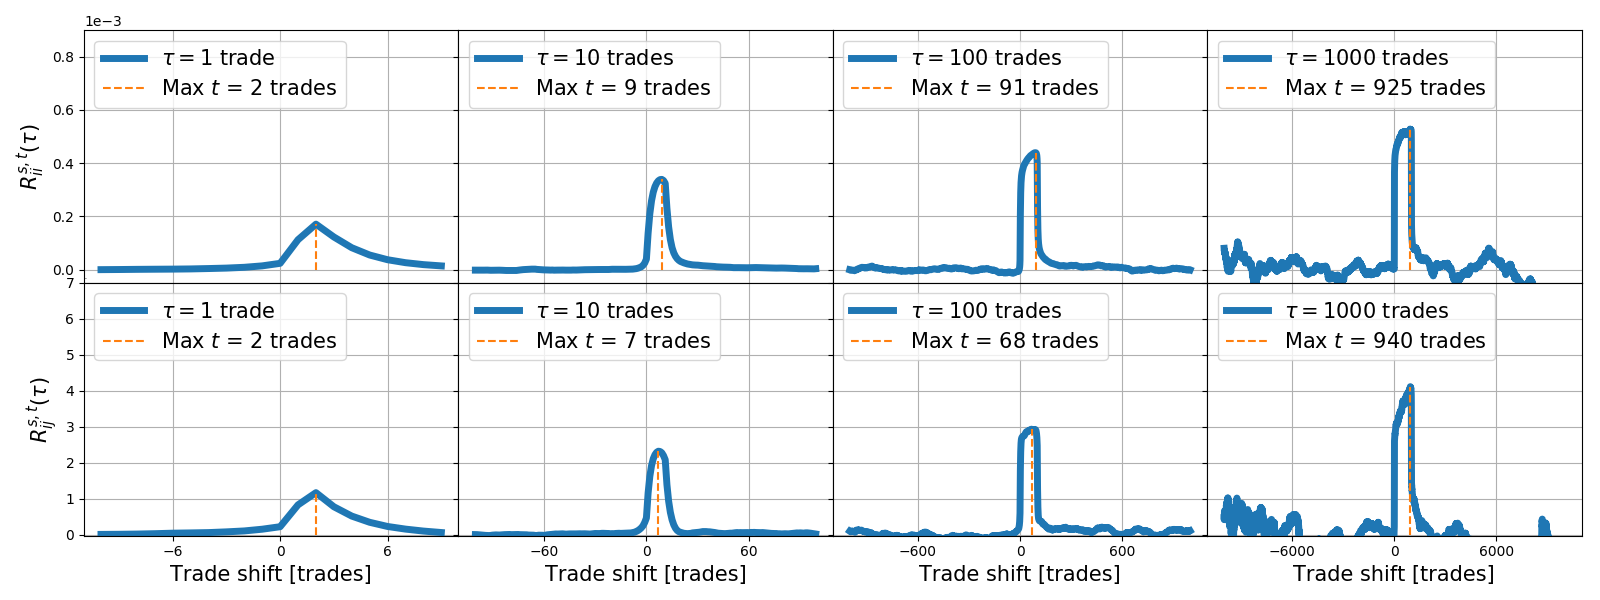
\includegraphics[width=\textwidth]{figures/04_shift_trade_RIG_APA.png}
    \caption{Self-response functions $R_{ii}^{t}\left(\tau\right)$ in 2008
             versus shift for the Transocean Ltd. stock (top) and
             cross-response functions $R_{ij}^{t}\left(\tau\right)$ excluding
             $\varepsilon^{t}_{j}\left(t\right) = 0$ in 2008 versus shift for
             the Transocean Ltd.-Apache Corp. stocks (bottom) in trade time
             scale.}
    \label{fig:shift_trade_scale}
\end{figure*}

In Fig. \ref{fig:shift_trade_scale}, it can be seen the response functions
results for fixed $\tau$ values while $t_{s}$ is variable. In the different
$\tau$ values figures, the results are almost the same. The response functions
are zero either if the time shift is larger than $\tau$, or if the time shift
is smaller than zero. For values between zero and $\tau$ there is a peak in a
position related to $\tau$. The response function grows and decrease relatively
fast. However, related on the time lag, there is a zone where the signal is
different to zero.

\begin{figure*}[htbp]
    \centering
    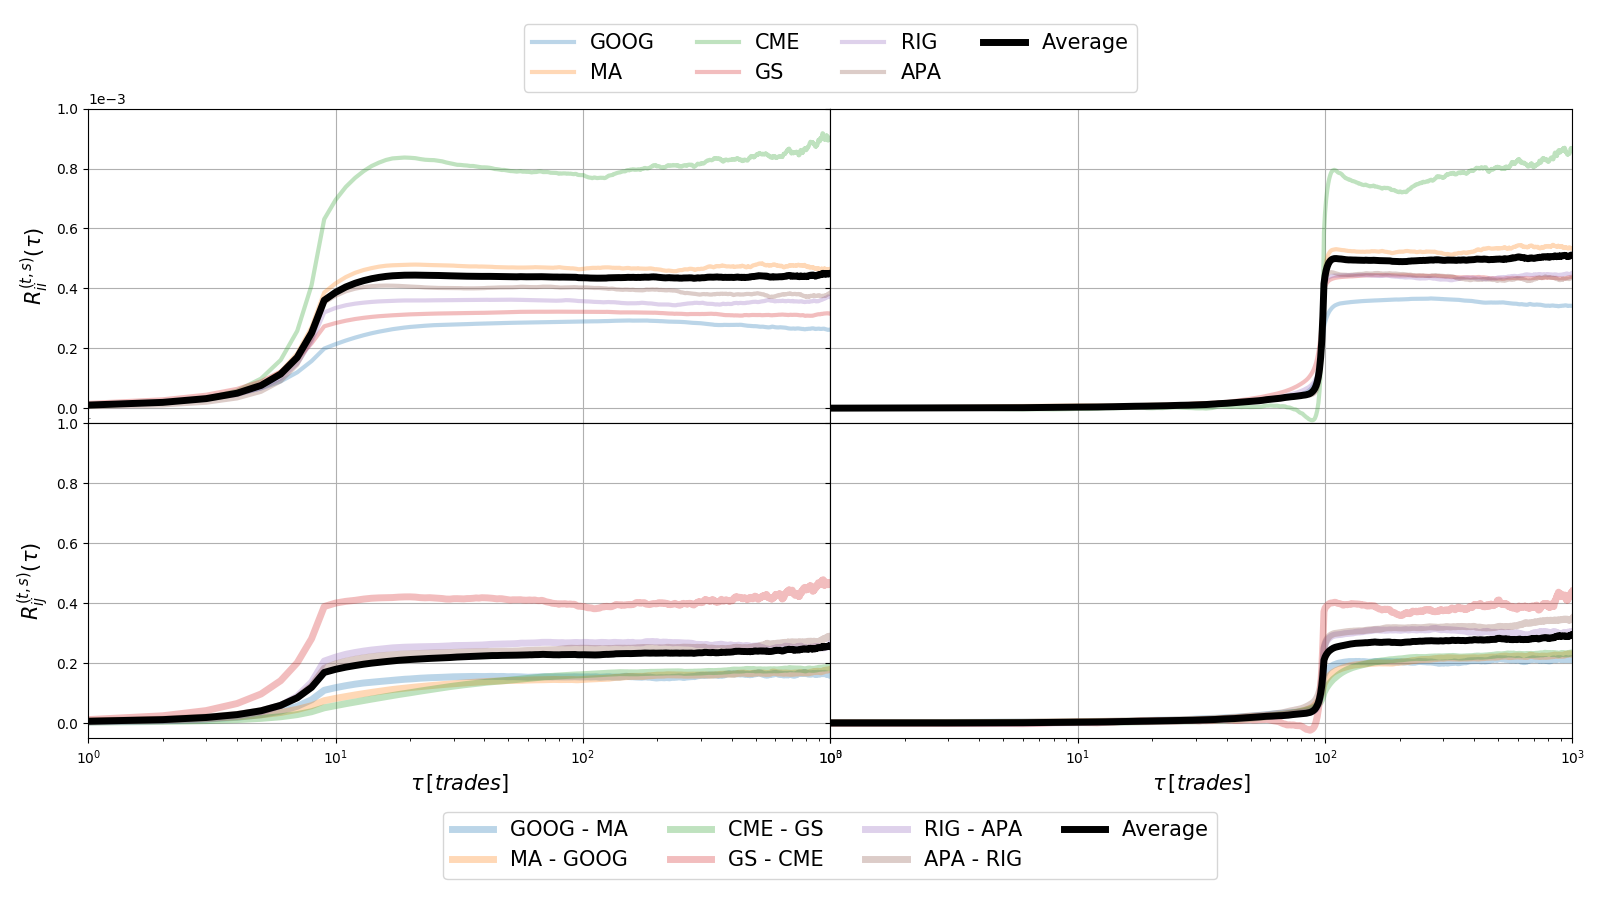
\includegraphics[width=\textwidth]{figures/04_shift_responses_trade.png}
    \caption{Self- and cross-response functions $R^{t}_{ij}\left(\tau\right)$
             in 2008 versus time lag $\tau$ on a logarithmic scale for
             different shifts in trade time scale. Self-response functions
             (left) of individual stocks and cross-response functions (right)
             of stocks pairs from the same economic sector.}
    \label{fig:shift_responses_trade_scale}
\end{figure*}

We tested the response function for fixed time shift values while $\tau$ is
variable. For every time shift (Fig. \ref{fig:shift_responses_trade_scale}),
both, self- and cross-response results are qualitatively the same. It can be
seen that the response functions have a zero signal before the time shift.
After the returns and trade signs find their corresponding order the signals
grow. In comparison with the values obtained in Fig.
\ref{fig:response_function_trade_scale}, it looks like the response function
values are stronger. However, this is an effect of the averaging of the
functions. As the returns and trade signs are shifted, they are less values to
average, and then the signals are stronger. Anyway, the figure shows the
importance of the relation between the trade signs and returns to compute the
response function.

%%%%%%%%%%%%%%%%%%%%%%%%%%%%%%%%%%%%%%%%%%%%%%%%%%%%%%%%%%%%%%%%%%%%%%%%%%%%%%%
\subsection{Physical time scale shift response functions}
\label{subsec:time_shift_physical}

In the physical time scale we compute the response function

\begin{equation}\label{eq:time_shift_physical}
    R_{ij}^{s, p}\left(\tau\right)=\left\langle r^{p}_{i}
    \left(t-t_{s},\tau\right) \cdot\varepsilon^{p}_{j}
    \left(t\right)\right\rangle _{t}
\end{equation}

\begin{figure*}[htbp]
    \centering
    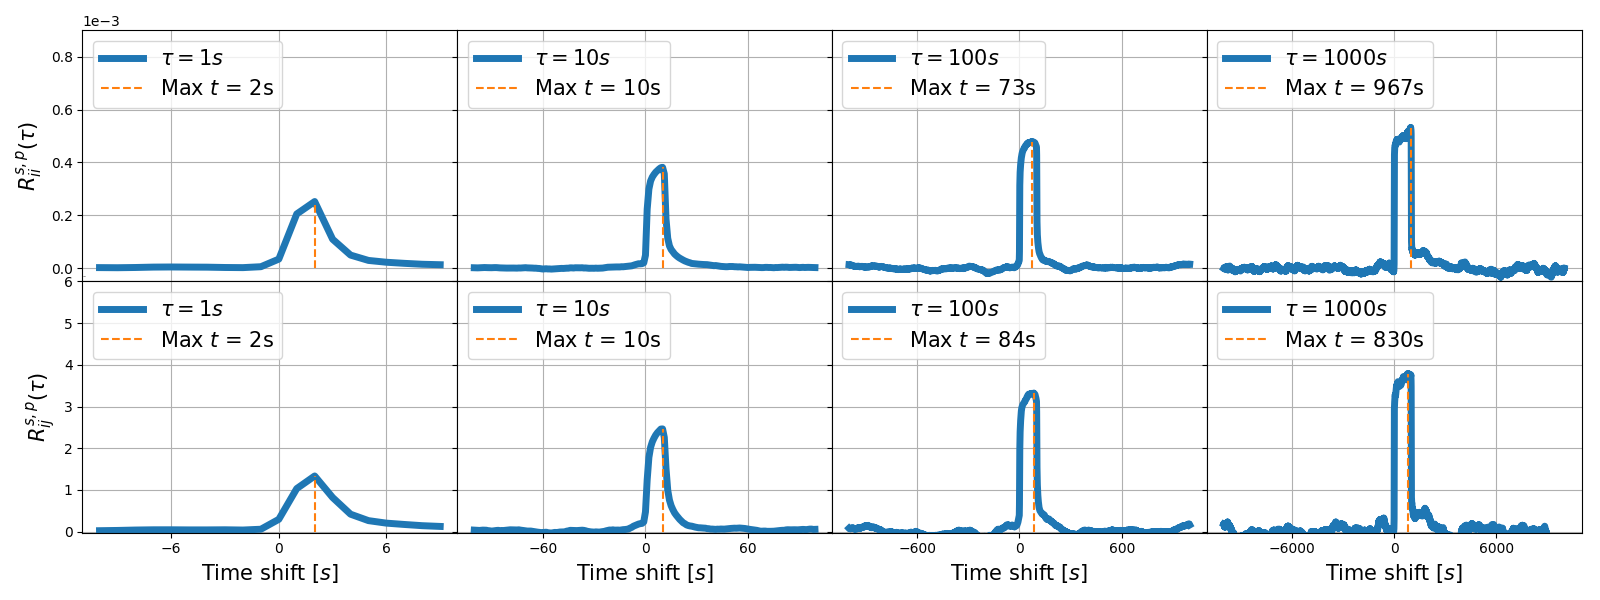
\includegraphics[width=\textwidth]{figures/04_shift_physical_RIG_APA.png}
    \caption{Self-response functions $R_{ii}^{p}\left(\tau\right)$ excluding
             $\varepsilon^{p}_{i}\left(t\right) = 0$ in 2008 versus shift for
             the Transocean Ltd. stock (top) and cross-response functions
             $R_{ij}^{p}\left(\tau\right)$ excluding
             $\varepsilon^{p}_{j}\left(t\right) = 0$ in 2008 versus shift for
             the Transocean Ltd.-Apache Corp. stocks (bottom) in physical time
             scale.}
    \label{fig:shift_physical_scale}
\end{figure*}

Similar to the results in Subsect. \ref{subsec:time_shift_trade}, Fig.
\ref{fig:shift_physical_scale} shows the responses functions for fixed $\tau$
values while $t_{s}$ is variable. Again, the response functions are zero if the
time shift is larger than the time lag, or if the time shift is smaller than
zero. For every $\tau$ value, there is a peak. The peak grows and decay
relatively fast. The response signal usually starts to grow in zero or a little
bit earlier and grows to a value around to $\tau$. In this zone the response
functions are different to zero.

\begin{figure*}[htbp]
    \centering
    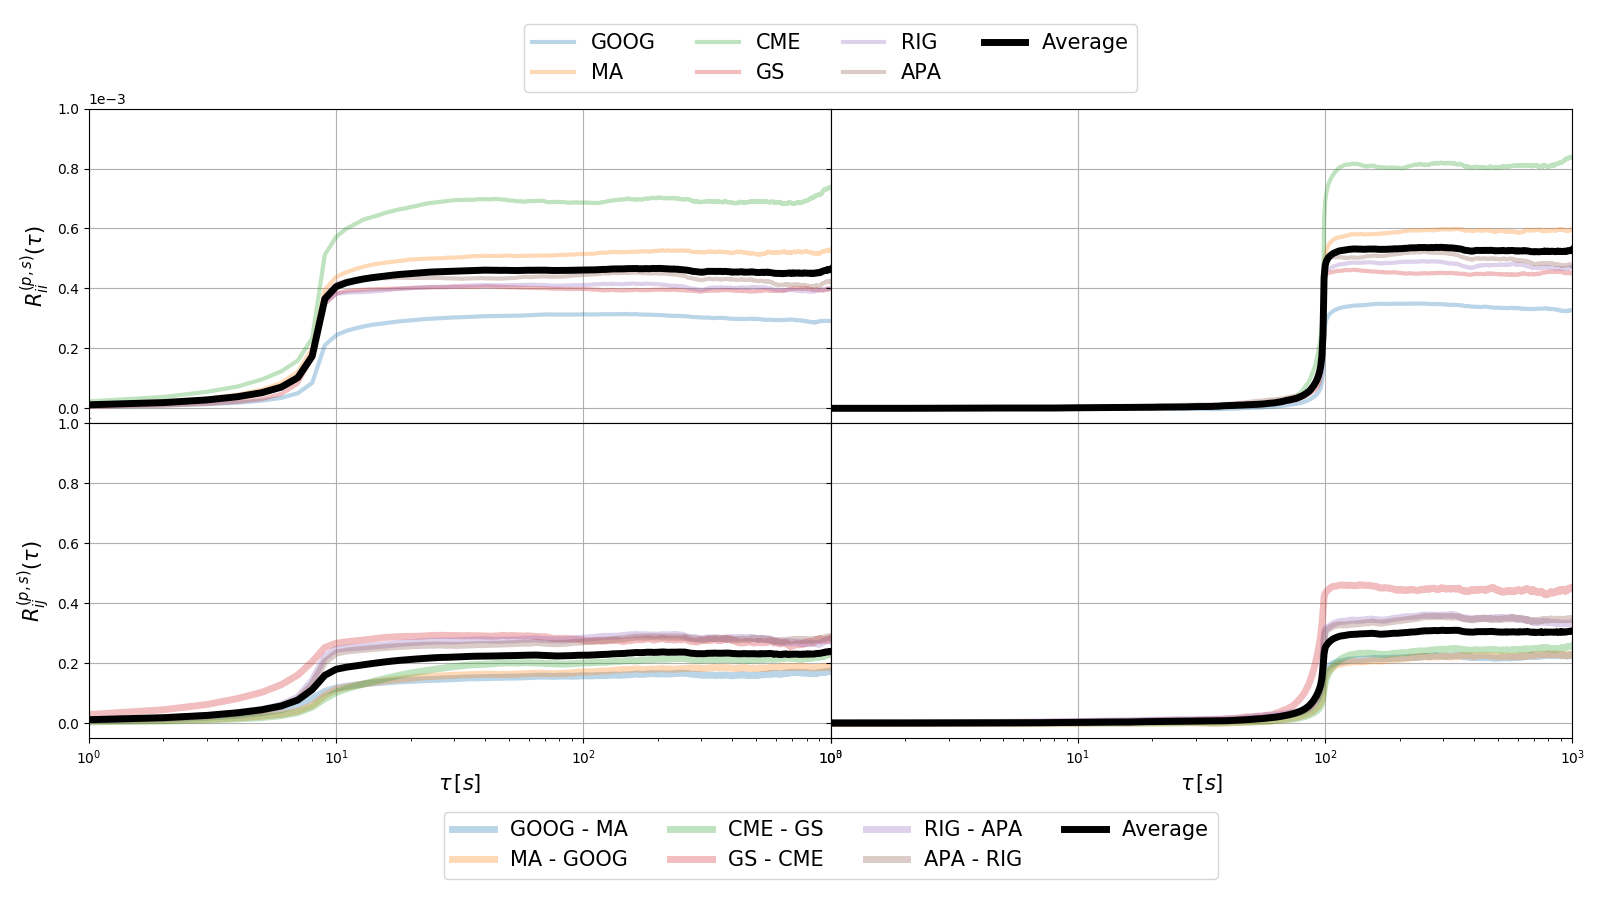
\includegraphics[width=\textwidth]{figures/04_shift_responses_physical.png}
    \caption{Self- and cross-response functions $R^{p}_{ij}\left(\tau\right)$
             excluding $\varepsilon^{p}_{j}\left(t\right) = 0$ in 2008 versus
             time lag $\tau$ on a logarithmic scale for different shifts in
             physical time scale. Self-responses functions (left) of individual
             stocks and cross-response functions (right) of stocks pairs from
             the same economic sector.}
    \label{fig:shift_responses_physical_scale}
\end{figure*}

The results for fixed time shift values and variable time lag are shown in Fig.
\ref{fig:shift_responses_physical_scale}. The self- and cross-response results
are qualitatively the same. As seen in the previous subsection, the response
functions are zero before the time shift value. After the returns and the trade
signs reach their order, the signals grow. The same effect of the apparent
stronger signal can be seen here, and again, it is due to the averaging values.

The results in trade time scale and physical time scale can be explained
understanding the dynamics of the market. A trade can or can not change the
price of a ticker. Therefore, when a change in price happens, a change in
midpoint price, and consequently in returns happens. Thus, it is extremely
important to keep the order of the events and the relation between them. When
we shift the trade signs and returns, this order is temporarily lost and as
outcome the signal does not have any meaningful information. When the order is
recovered during the shift, the signal grows again, showing response function
values different to zero. In this section we were interested only in the order
(shift) and not in the responses values, which were analyzed in Sect.
\ref{sec:response_functions_imp}.

Then the question is what is the ideal time shift to compute the response
functions. Our approach in Sect. \ref{sec:response_functions_imp} takes in account
that the changes in the quotes are the ones that attract the agents to buy or
sell their shares. Hence, they directly impact the trade signs. According to
the results, the response can take up to two time steps in the corresponding
scale to react to the change in quotes. Thus, a time shift larger than two time
steps makes no sense.
On the other hand, in the case of the physical time scale, where a sampling is
used, to assure the selection of a midpoint price at the beginning of a second,
it is a good strategy to use the last midpoint of the previous second as the
first midpoint price of the current second. In this case an apparent one second
shift is used between returns and trade signs.